\documentclass{extbook}[14pt]
\usepackage{multicol, enumerate, enumitem, hyperref, color, soul, setspace, parskip, fancyhdr, amssymb, amsthm, amsmath, bbm, latexsym, units, mathtools}
\everymath{\displaystyle}
\usepackage[headsep=0.5cm,headheight=0cm, left=1 in,right= 1 in,top= 1 in,bottom= 1 in]{geometry}
\usepackage{dashrule}  % Package to use the command below to create lines between items
\newcommand{\litem}[1]{\item #1

\rule{\textwidth}{0.4pt}}
\pagestyle{fancy}
\lhead{}
\chead{Answer Key for Progress Quiz 8 Version C}
\rhead{}
\lfoot{4553-3922}
\cfoot{}
\rfoot{Fall 2020}
\begin{document}
\textbf{This key should allow you to understand why you choose the option you did (beyond just getting a question right or wrong). \href{https://xronos.clas.ufl.edu/mac1105spring2020/courseDescriptionAndMisc/Exams/LearningFromResults}{More instructions on how to use this key can be found here}.}

\textbf{If you have a suggestion to make the keys better, \href{https://forms.gle/CZkbZmPbC9XALEE88}{please fill out the short survey here}.}

\textit{Note: This key is auto-generated and may contain issues and/or errors. The keys are reviewed after each exam to ensure grading is done accurately. If there are issues (like duplicate options), they are noted in the offline gradebook. The keys are a work-in-progress to give students as many resources to improve as possible.}

\rule{\textwidth}{0.4pt}

\begin{enumerate}\litem{
Determine the domain of the function below.
\[ f(x) = \frac{5}{25x^{2} +55 x + 30} \]

The solution is \( \text{All Real numbers except } x = -1.200 \text{ and } x = -1.000. \), which is option E.\begin{enumerate}[label=\Alph*.]
\item \( \text{All Real numbers except } x = a, \text{ where } a \in [-1.43, -1.16] \)

All Real numbers except $x = -1.200$, which corresponds to removing only 1 value from the denominator.
\item \( \text{All Real numbers except } x = a \text{ and } x = b, \text{ where } a \in [-30.2, -29.61] \text{ and } b \in [-25.05, -24.65] \)

All Real numbers except $x = -30.000$ and $x = -25.000$, which corresponds to not factoring the denominator correctly.
\item \( \text{All Real numbers except } x = a, \text{ where } a \in [-30.2, -29.61] \)

All Real numbers except $x = -30.000$, which corresponds to removing a distractor value from the denominator.
\item \( \text{All Real numbers.} \)

This corresponds to thinking the denominator has complex roots or that rational functions have a domain of all Real numbers.
\item \( \text{All Real numbers except } x = a \text{ and } x = b, \text{ where } a \in [-1.43, -1.16] \text{ and } b \in [-1.04, -0.29] \)

All Real numbers except $x = -1.200$ and $x = -1.000$, which is the correct option.
\end{enumerate}

\textbf{General Comment:} Recall that dividing by zero is not a real number. Therefore the domain is all real numbers \textbf{except} those that make the denominator 0.
}
\litem{
Solve the rational equation below. Then, choose the interval(s) that the solution(s) belongs to.
\[ \frac{-5}{9x -2} + 9 = \frac{5}{-63x + 14} \]

The solution is \( x = 0.275 \), which is option B.\begin{enumerate}[label=\Alph*.]
\item \( \text{All solutions lead to invalid or complex values in the equation.} \)

This corresponds to thinking $x = 0.275$ leads to dividing by zero in the original equation, which it does not.
\item \( x \in [0.28,1.28] \)

* $x = 0.275$, which is the correct option.
\item \( x_1 \in [0, 0.7] \text{ and } x_2 \in [0.28,0.41] \)

$x = 0.275 \text{ and } x = 0.346$, which corresponds to getting the correct solution and believing there should be a second solution to the equation.
\item \( x \in [-0.7,0] \)

$x = -0.169$, which corresponds to not distributing the factor $9x -2$ correctly when trying to eliminate the fraction.
\item \( x_1 \in [-0.7, 0] \text{ and } x_2 \in [0.26,0.31] \)

$x = -0.169 \text{ and } x = 0.275$, which corresponds to getting the correct solution and believing there should be a second solution to the equation.
\end{enumerate}

\textbf{General Comment:} Distractors are different based on the number of solutions. Remember that after solving, we need to make sure our solution does not make the original equation divide by zero!
}
\litem{
Solve the rational equation below. Then, choose the interval(s) that the solution(s) belongs to.
\[ \frac{-4x}{-5x + 5} + \frac{-6x^{2}}{25x^{2} +5 x -30} = \frac{6}{-5x -6} \]

The solution is \( \text{There are two solutions: } x = 0.493 \text{ and } x = -4.350 \), which is option D.\begin{enumerate}[label=\Alph*.]
\item \( x \in [-2.6,-0.3] \)


\item \( x \in [-7.5,-2.7] \)


\item \( \text{All solutions lead to invalid or complex values in the equation.} \)


\item \( x_1 \in [0.1, 1] \text{ and } x_2 \in [-6.35,-0.35] \)

* $x = 0.493 \text{ and } x = -4.350$, which is the correct option.
\item \( x_1 \in [0.1, 1] \text{ and } x_2 \in [-1,4] \)


\end{enumerate}

\textbf{General Comment:} Distractors are different based on the number of solutions. Remember that after solving, we need to make sure our solution does not make the original equation divide by zero!
}
\litem{
Choose the graph of the equation below.
\[ f(x) = \frac{1}{(x - 1)^2} + 2 \]

The solution is the graph below, which is option D.
\begin{center}
    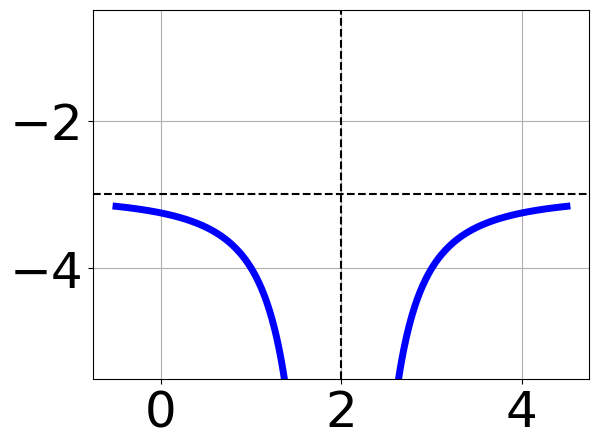
\includegraphics[width=0.3\textwidth]{../Figures/rationalEquationToGraphCopyDC.png}
\end{center}\begin{enumerate}[label=\Alph*.]
\begin{multicols}{2}
\item 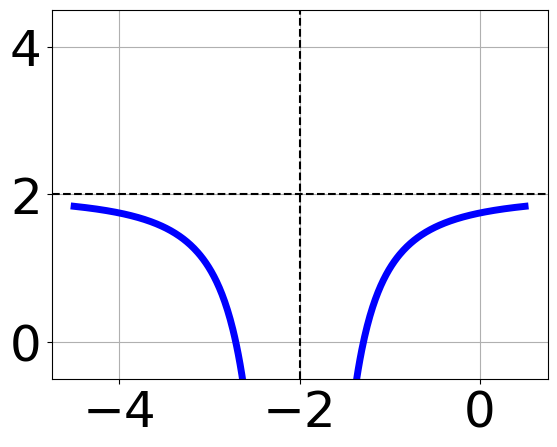
\includegraphics[width = 0.3\textwidth]{../Figures/rationalEquationToGraphCopyAC.png}
\item 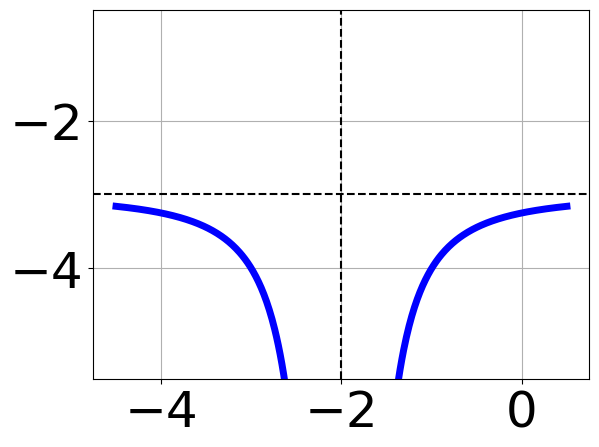
\includegraphics[width = 0.3\textwidth]{../Figures/rationalEquationToGraphCopyBC.png}
\item 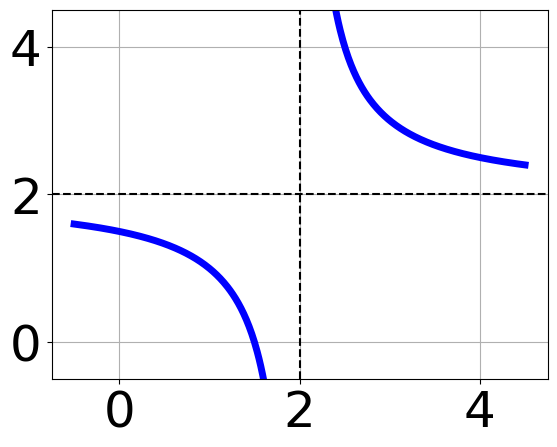
\includegraphics[width = 0.3\textwidth]{../Figures/rationalEquationToGraphCopyCC.png}
\item 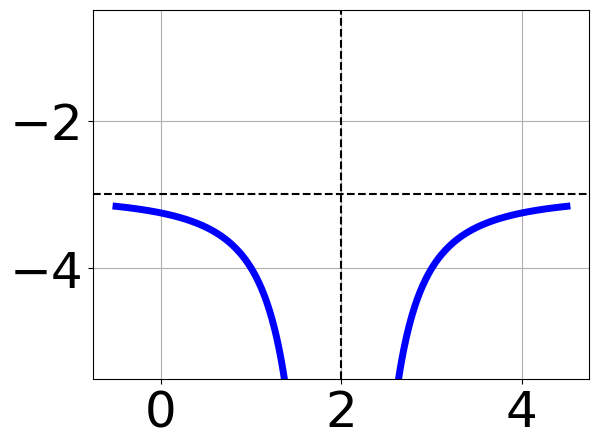
\includegraphics[width = 0.3\textwidth]{../Figures/rationalEquationToGraphCopyDC.png}
\end{multicols}\item None of the above.\end{enumerate}
\textbf{General Comment:} Remember that the general form of a basic rational equation is $ f(x) = \frac{a}{(x-h)^n} + k$, where $a$ is the leading coefficient (and in this case, we assume is either $1$ or $-1$), $n$ is the degree (in this case, either $1$ or $2$), and $(h, k)$ is the intersection of the asymptotes.
}
\litem{
Choose the equation of the function graphed below.

\begin{center}
    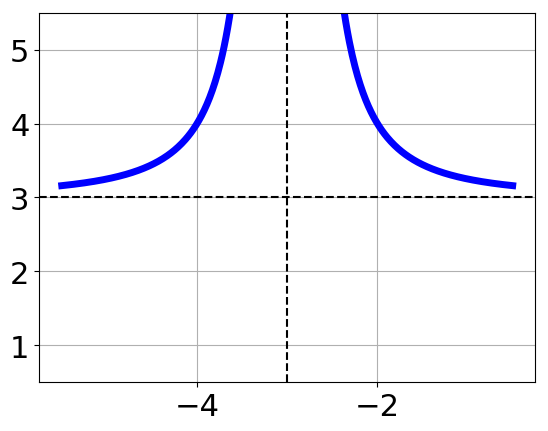
\includegraphics[width=0.5\textwidth]{../Figures/rationalGraphToEquationC.png}
\end{center}




The solution is \( \text{None of the above as it should be } f(x) = \frac{-1}{(x + 3)^2} + 2 \), which is option E.\begin{enumerate}[label=\Alph*.]
\item \( f(x) = \frac{-1}{x - 3} + 2 \)

Corresponds to thinking the graph was a shifted version of $\frac{1}{x}$.
\item \( f(x) = \frac{-1}{(x - 3)^2} + 2 \)

The $x$-value of the equation does not match the graph.
\item \( f(x) = \frac{1}{(x + 3)^2} + 2 \)

Corresponds to using the general form $f(x) = \frac{a}{(x-h)^2}+k$ and the opposite leading coefficient.
\item \( f(x) = \frac{1}{x + 3} + 2 \)

Corresponds to thinking the graph was a shifted version of $\frac{1}{x}$, using the general form $f(x) = \frac{a}{(x-h)^2}+k$, and the opposite leading coefficient.
\item \( \text{None of the above} \)

None of the equation options were the correct equation.
\end{enumerate}

\textbf{General Comment:} Remember that the general form of a basic rational equation is $ f(x) = \frac{a}{(x-h)^n} + k$, where $a$ is the leading coefficient (and in this case, we assume is either $1$ or $-1$), $n$ is the degree (in this case, either $1$ or $2$), and $(h, k)$ is the intersection of the asymptotes.
}
\litem{
Choose the graph of the equation below.
\[ f(x) = \frac{-1}{(x + 2)^2} + 2 \]

The solution is the graph below, which is option E.
\begin{center}
    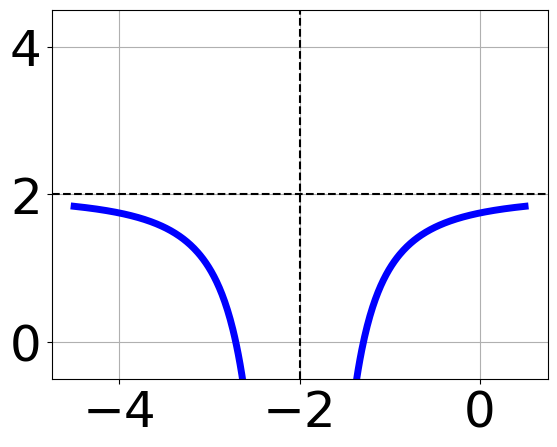
\includegraphics[width=0.3\textwidth]{../Figures/rationalEquationToGraphEC.png}
\end{center}\begin{enumerate}[label=\Alph*.]
\begin{multicols}{2}
\item 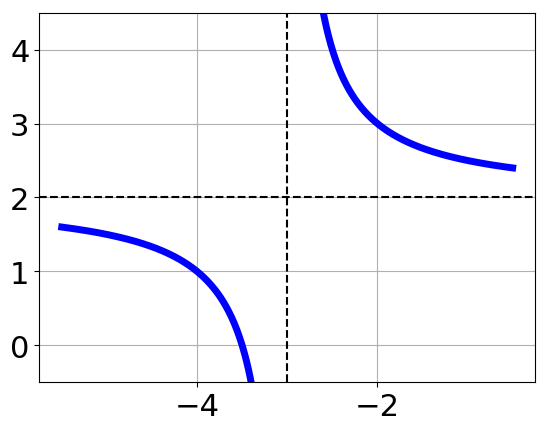
\includegraphics[width = 0.3\textwidth]{../Figures/rationalEquationToGraphAC.png}
\item 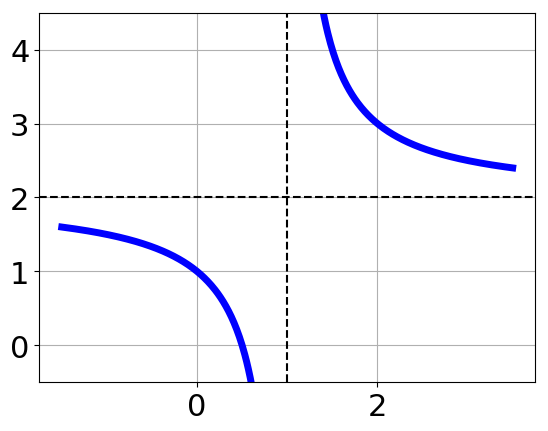
\includegraphics[width = 0.3\textwidth]{../Figures/rationalEquationToGraphBC.png}
\item 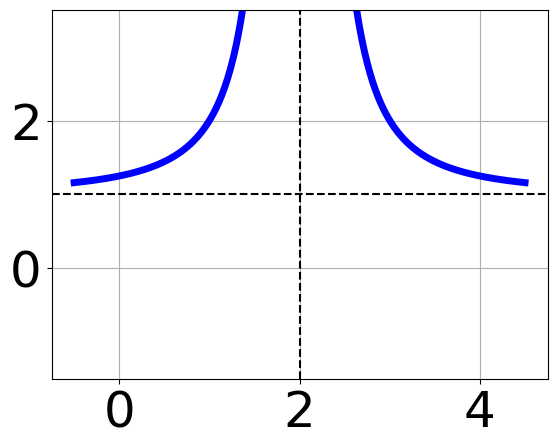
\includegraphics[width = 0.3\textwidth]{../Figures/rationalEquationToGraphCC.png}
\item 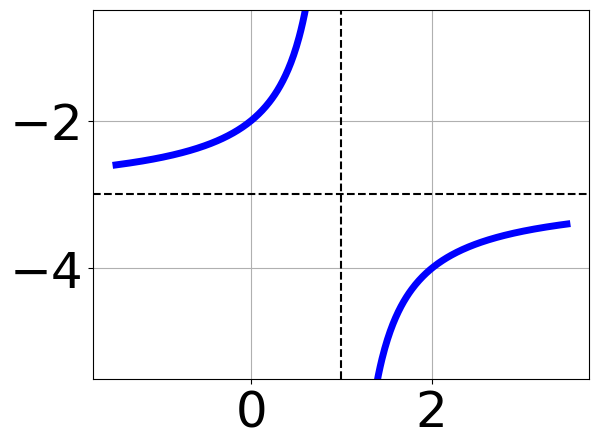
\includegraphics[width = 0.3\textwidth]{../Figures/rationalEquationToGraphDC.png}
\end{multicols}\item None of the above.\end{enumerate}
\textbf{General Comment:} Remember that the general form of a basic rational equation is $ f(x) = \frac{a}{(x-h)^n} + k$, where $a$ is the leading coefficient (and in this case, we assume is either $1$ or $-1$), $n$ is the degree (in this case, either $1$ or $2$), and $(h, k)$ is the intersection of the asymptotes.
}
\litem{
Solve the rational equation below. Then, choose the interval(s) that the solution(s) belongs to.
\[ \frac{6x}{-6x -6} + \frac{-4x^{2}}{30x^{2} +48 x + 18} = \frac{4}{-5x -3} \]

The solution is \( \text{There are two solutions: } x = -0.757 \text{ and } x = 0.933 \), which is option D.\begin{enumerate}[label=\Alph*.]
\item \( x_1 \in [-2.26, -0.66] \text{ and } x_2 \in [-7,0] \)


\item \( x \in [0.19,2.22] \)


\item \( \text{All solutions lead to invalid or complex values in the equation.} \)


\item \( x_1 \in [-2.26, -0.66] \text{ and } x_2 \in [0.93,5.93] \)

* $x = -0.757 \text{ and } x = 0.933$, which is the correct option.
\item \( x \in [-0.63,-0.06] \)


\end{enumerate}

\textbf{General Comment:} Distractors are different based on the number of solutions. Remember that after solving, we need to make sure our solution does not make the original equation divide by zero!
}
\litem{
Choose the equation of the function graphed below.

\begin{center}
    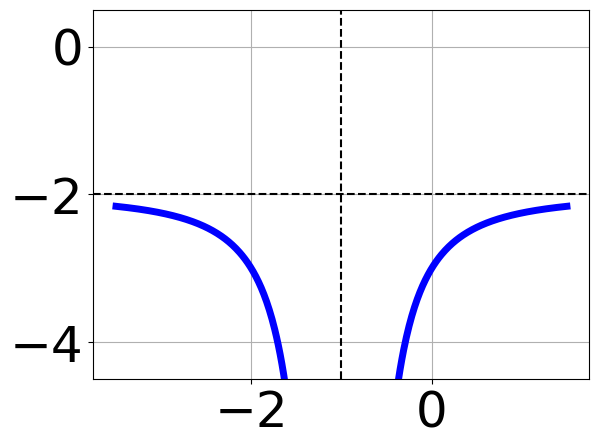
\includegraphics[width=0.5\textwidth]{../Figures/rationalGraphToEquationCopyC.png}
\end{center}




The solution is \( f(x) = \frac{-1}{x + 1} + 2 \), which is option B.\begin{enumerate}[label=\Alph*.]
\item \( f(x) = \frac{-1}{(x + 1)^2} + 2 \)

Corresponds to thinking the graph was a shifted version of $\frac{1}{x^2}$.
\item \( f(x) = \frac{-1}{x + 1} + 2 \)

This is the correct option.
\item \( f(x) = \frac{1}{x - 1} + 2 \)

Corresponds to using the general form $f(x) = \frac{a}{x+h}+k$ and the opposite leading coefficient.
\item \( f(x) = \frac{1}{(x - 1)^2} + 2 \)

Corresponds to thinking the graph was a shifted version of $\frac{1}{x^2}$, using the general form $f(x) = \frac{a}{x+h}+k$, and the opposite leading coefficient.
\item \( \text{None of the above} \)

This corresponds to believing the vertex of the graph was not correct.
\end{enumerate}

\textbf{General Comment:} Remember that the general form of a basic rational equation is $ f(x) = \frac{a}{(x-h)^n} + k$, where $a$ is the leading coefficient (and in this case, we assume is either $1$ or $-1$), $n$ is the degree (in this case, either $1$ or $2$), and $(h, k)$ is the intersection of the asymptotes.
}
\litem{
Determine the domain of the function below.
\[ f(x) = \frac{4}{30x^{2} -48 x + 18} \]

The solution is \( \text{All Real numbers except } x = 0.600 \text{ and } x = 1.000. \), which is option E.\begin{enumerate}[label=\Alph*.]
\item \( \text{All Real numbers except } x = a \text{ and } x = b, \text{ where } a \in [14.83, 15.94] \text{ and } b \in [35.83, 36.19] \)

All Real numbers except $x = 15.000$ and $x = 36.000$, which corresponds to not factoring the denominator correctly.
\item \( \text{All Real numbers except } x = a, \text{ where } a \in [14.83, 15.94] \)

All Real numbers except $x = 15.000$, which corresponds to removing a distractor value from the denominator.
\item \( \text{All Real numbers.} \)

This corresponds to thinking the denominator has complex roots or that rational functions have a domain of all Real numbers.
\item \( \text{All Real numbers except } x = a, \text{ where } a \in [0.43, 0.72] \)

All Real numbers except $x = 0.600$, which corresponds to removing only 1 value from the denominator.
\item \( \text{All Real numbers except } x = a \text{ and } x = b, \text{ where } a \in [0.43, 0.72] \text{ and } b \in [0.7, 1.44] \)

All Real numbers except $x = 0.600$ and $x = 1.000$, which is the correct option.
\end{enumerate}

\textbf{General Comment:} Recall that dividing by zero is not a real number. Therefore the domain is all real numbers \textbf{except} those that make the denominator 0.
}
\litem{
Solve the rational equation below. Then, choose the interval(s) that the solution(s) belongs to.
\[ \frac{3}{5x -9} + 5 = \frac{4}{-40x + 72} \]

The solution is \( x = 1.660 \), which is option E.\begin{enumerate}[label=\Alph*.]
\item \( x_1 \in [-3.94, -0.94] \text{ and } x_2 \in [1.65,1.71] \)

$x = -1.940 \text{ and } x = 1.660$, which corresponds to getting the correct solution and believing there should be a second solution to the equation.
\item \( x \in [-3.94,-0.94] \)

$x = -1.940$, which corresponds to not distributing the factor $5x -9$ correctly when trying to eliminate the fraction.
\item \( \text{All solutions lead to invalid or complex values in the equation.} \)

This corresponds to thinking $x = 1.660$ leads to dividing by zero in the original equation, which it does not.
\item \( x_1 \in [1.66, 2.66] \text{ and } x_2 \in [1.79,2.05] \)

$x = 1.660 \text{ and } x = 1.840$, which corresponds to getting the correct solution and believing there should be a second solution to the equation.
\item \( x \in [1.66,2.66] \)

* $x = 1.660$, which is the correct option.
\end{enumerate}

\textbf{General Comment:} Distractors are different based on the number of solutions. Remember that after solving, we need to make sure our solution does not make the original equation divide by zero!
}
\end{enumerate}

\end{document}